\subsection{Ordered Pairs and Cartesian Products}

\begin{tcolorbox}[title=Problem 5, breakable]
    Prove parts $2$ and $3$ of Theorem $4.13$.
\end{tcolorbox}

\begin{proof}
    Show $A \times (B \cup C) = (A \times B) \cup (A \times C)$.

    Let $p$ be an arbitrary element in $A \times (B \cup C)$. Let $(x, y) = p$.
    Clearly $x \in A$ and $y \in (B \cup C)$. It follows that $y \in B$ or $y \in
        C$. Suppose $y \in B$. Then $x \in A$ and $y \in B$ so $p \in A \times B$.
    Suppose $y \in C$. Then $x \in A$ and $y \in C$ so $p \in A \times C$. So, $p
        \in A \times B$ or $p \in A \times C$. It follows that $p \in (A \times B) \cup
        (A \times C)$.

    Let $p$ be an arbitrary element in $(A \times B) \cup (A \times C)$. It follows
    that $p \in A \times B$ or $p \in A \times C$. Let $(x, y) = p$. Clearly $x \in
        A$ and $y$ is in $B$ or $C$. It follows that $p \in A \times (B \cup C)$.
\end{proof}

\begin{proof}
    Show $(A \times B) \cap (C \times D) = (A \cap C) \times (B \cap D)$.

    Let $p$ be an arbitrary element in $(A \times B) \cap (C \times D)$. It follows
    that $p \in A \times B$ and $p \in C \times D$. Let $(x, y) = p$. Then, $(x, y)
        \in A \times B$ and $(x, y) \in C \times D$. So, $x \in A$ and $x \in C$.
    Therefore, $x \in A \cap C$. Also, $y \in B$ and $y \in D$. Therefore $y \in B
        \cap D$. Since, $x \in A \cap C$ and $y \in B \cap D$, $p \in (A \cap C) \times
        (B \cap D)$.

    Let $p$ be an arbitrary element in $(A \cap C) \times (B \cap D)$. Let $(x, y)
        = p$. Then, $x \in A \cap C$ and $y \in B \cap D$. Since $x \in A \cap C$, $x
        \in A$ and $x \in C$. Since $y \in B \cap D$, $y \in B$ and $y \in D$. Since $x
        \in A$ and $y \in B$, $p \in A \times B$. Since $x \in C$ and $y \in D$, $p \in
        C \times D$. S ince $p \in A \times B$ and $p \in C \times D$, $p \in (A \times
        B) \cap (C \times D)$.
\end{proof}

\begin{tcolorbox}[title=Problem 6, breakable]
    What's wrong with the following proof that for any sets $A$, $B$, $C$, and $D$,
    $(A \cup C) \times (B \cup D) \subseteq (A \times B) \cup (C \times D)$?
    (Note that this is the reverse of the inclusion in part $4$ of Theorem $4.1.3$)

    \begin{proof}
        Suppose $(x, y) \in (A \cup C) \times (B \cup D)$.Then $x \in A \cup C$.
        and $y \in B \cup D$, so either $x \in A$ or $x \in C$, 
        and either $y \in B$ or $y \in D$. We consider these cases seperately.

        Case 1. $x \in A$ and $y \in B$. Then $(x, y) \in A \times B$.

        Case 2. $x \in C$ and $y \in D$. Then $(x, y) \in C \times D$.

        Thus, either $(x, y) \in A \times B$ or $(x, y) \in C \times D$, so $(x, y) \in
            (A \times B) \cup (C \times D)$.
    \end{proof}
\end{tcolorbox}

\textbf{Solution}

The proof doesn't account for all cases namely, $x \in A$ and $y \in D$ or $x
    \in C$ and $y \in B$.

\begin{tcolorbox}[title=Problem 7, breakable]
    If $A$ has $m$ elements and $B$ has $n$ elements, how many elements does $A \times B$ have?
\end{tcolorbox}

\textbf{Solution}

$A \times B$ has $m \cdot n$ elements.

\begin{tcolorbox}[title=Problem 12, breakable]
    Prove that for any sets $A$, $B$, $C$, and $D$, if $A \times B$ and $C \times D$ are disjoint,
    then either $A$ and $C$ are disjoint or $B$ and $D$ are disjoint.
\end{tcolorbox}

\begin{proof}
    For contradiction, suppose $A \times B$ and $C \times D$ are disjoint
    and $A$ and $C$ are not disjoint and $B$ and $D$ are not disjoint.
    Let $x$ be an element of $A \cap C \not= \emptyset$.
    Let $y$ be an element of $B \cap D \not= \emptyset$.
    Let $p = (x, y)$. Since $x \in A$ and $y \in B$, $p \in A \times B$.
    Since $x \in C$ and $y \in D$, $p \in C \times D$.
    It follows that $p \in (A \times B) \cap (C \times D)$ contradicting the disjointness of $A \times B$ and $C \times D$.
\end{proof}

\begin{tcolorbox}[title=Problem 13, breakable]
    Suppose $I \not= \emptyset$. Prove that for any indexed family of sets $\{ A_i \mid i \in I\}$
    and any set $B$, $(\bigcap_{i \in I} A_i) \times B = \bigcap_{i \in I}(A_i \times B)$. Where
    in the proof does the assumption that $I \not= \emptyset$ get used?
\end{tcolorbox}

For the intersection operation to be defined the set must not be emtpy (More
operations on sets $15$ b).

\begin{proof}
    Let $p$ be an arbitrary element in $(\bigcap_{i \in I} A_i) \times B$.
    Let $(x, y) = p$.
    Notice $x \in A_i$ for all $i \in I$ and $y \in B$.
    It follows that $p \in A_i \times B$ for all $i \in I$.
    So $p \in \bigcap_{i \in I}(A_i \times B)$.

    Let $p$ be an arbitrary element in $\bigcap_{i \in I}(A_i \times B)$. Notice $p
        \in A_i \times B$ for all $i \in I$. Let $(x, y) = p$. It follows that $x \in
        A_i$ for all $i \in I$. Therefore $x \in \bigcap_{i \in I} A_i$. Since $y \in
        B$, it follows that $p \in \bigcap_{i \in I}(A_i) \times B$.
\end{proof}

\begin{tcolorbox}[title=Problem 15, breakable]
    This problem was suggested by Professor Alan Taylor of Union College, NY.
    Consider the following putative theorem.

    \textbf{Theorem?} \emph{For any sets $A$, $B$, $C$, and $D$, if $A \times B \subseteq C \times D$
        then $A \subseteq C$ and $B \subseteq D$.}

    Is the following proof correct? If so, what proof strategies does it use? If
    not, can it be fixed? Is the theorem correct?

    \begin{proof}
        Suppose $A \times B \subseteq C \times D$. Let $a$ be an arbitrary element of $A$
        and let $b$ be an arbitrary element of $B$. Then $(a, b) \in A \times B$, so 
        since $A \times B \subseteq C \times D$, $(a, b) \in C \times D$.
        Therefore $a \in C$ and $b \in D$. Since $a$ and $b$ were arbitrary elements of $A$ and $B$,
        respectively, this shows $A \subseteq C$ and $B \subseteq D$.
    \end{proof}
\end{tcolorbox}

\textbf{Solution:}

The proof is incorrect. It implicitly assumes The sets $A$ and $B$ are not
empty. It can be fixed by assuming $A$ and $B$ are not empty. The theorem is
incorrect.

\subsection{Relations}

\begin{tcolorbox}[title=Problem 1, breakable]
    (a) $\{(p, q) \in P \times P \mid \text{ the person $p$ is a parent of person $q$}\}$,
    where $P$ is the set of all living people.

    (b) $\{(x, y) \in \mathcal{R}^2 \mid y > x^2\}$
\end{tcolorbox}

\textbf{Solution (a):}

Domain: People who have children that are alive.

Range: People whose parents are still living.

\textbf{Solution (b):}

Domain: All $x \in \mathcal{R}$.

Range: All $y > 0$.

\begin{tcolorbox}[title=Problem 5, breakable]
    Suppose that $A = \{1, 2, 3\}, B = \{4, 5, 6\},
        R = \{(1, 4), (1, 5), (2, 5), (3, 6)\}, \text{ and } S = \{(4, 5), (4, 6), (5, 4), (6, 6)\}$.
    Note that $R$ is a relation from $A$ to $B$ and $S$ is a relation from $B$ to $B$. 
    Find the following relations:

    (a) $S \circ R$.

    (b) $S \circ S^{-1}$.
\end{tcolorbox}

\textbf{Solution (a):}

$S \circ R = \{(1, 5), (1, 6), (1, 4), (2, 4), (3, 6)\}$

\textbf{Solution (b):}

$S \circ S^{-1} = \{(5, 5), (5, 6), (6, 6), (6, 5), (4, 4)\}$

\begin{tcolorbox}[title=Problem 7, breakable]
    (a) Prove part $3$ of Theorem $4.2.5$ by imitating the proof of part $2$ in the text.

    (b) Give an alternative proof of part $3$ of Theorem $4.2.5$ by showing that it follows 
    from part $1$ and $2$.

    (c) Complete the proof of part $4$ of Theorem $4.2.5$.

    (d) Prove part $5$of Theorem $4.2.5$.
\end{tcolorbox}

\textbf{(a) We want to prove that } $Ran(R^{-1}) = Dom(R)$.

\begin{proof} 
    \begin{align*}
        a \in Ran(R^{-1}) \iff & \exists{b \in B}((b, a) \in R^{-1}) \\
        \iff                   & \exists{b \in B}((a, b) \in R)      \\
        \iff                   & a \in Dom(R)
    \end{align*}
\end{proof}

\textbf{(b) We want to prove that } $Ran(R^{-1}) = Dom(R)$ \textbf{ using parts (1) and (2).}

\begin{proof}
    Let $a$ be an arbitrary element in $Ran(R^{-1})$.
    By part $2$ $a \in Ran(R^{-1}) \iff a \in Dom({(R^{-1})}^{-1})$.
    By part $1$ $a \in Dom({(R^{-1})}^{-1}) \iff a \in Dom(R)$.
\end{proof}

\textbf{(c) We want to prove that } $(T \circ S) \circ R = T \circ (S \circ R)$.

\begin{proof}
    Let $(a, d)$ be an arbitrary pair of elements in $(T \circ S) \circ R$.
    There exists $c$ such that $(a, c) \in R$ and $(c, d) \in (T \circ S)$.
    There exists $b$ such that $(c, b) \in S$ and $(b, d) \in T$.
    Since $(a, c) \in R$ and $(c, b) \in S$, $(a, b) \in S \circ R$.
    Since $(a, b) \in S \circ R$ and $(b, d) \in T$, $(a, d) \in T \circ (S \circ R)$.
\end{proof}

\textbf{(d) We want to prove that } ${(S \circ R)}^{-1} = R^{-1} \circ S^{-1}$.

\begin{proof}
    Let $(y, x)$ be an arbitrary pair of elements in ${(S \circ R)}^{-1}$.
    Then $(x, y) \in S \circ R$. There exists $c$ such that $(x, c) \in R$ and $(c, y) \in S$.
    So $(c, x) \in R^{-1}$ and $(y, c) \in S^{-1}$.
    It follows that $(y, x) \in R^{-1} \circ S^{-1}$.

    Let $(y, x)$ be an arbitrary pair of elements in $R^{-1} \circ S^{-1}$. There
    exists $c$ such that $(y, c) \in S^{-1}$ and $(c, x) \in R^{-1}$. Then $(c, y)
        \in S$ and $(x, c) \in R$. So $(x, y) \in S \circ R$ and $(y, x) \in {(S \circ
            R)}^{-1}$.
\end{proof}

\begin{tcolorbox}[title=Problem 8, breakable]
    Let $E = \{(p, q) \in P \times P \mid \text{ the person $p$ is an enemy of the person $q$}\}$,
    and $F = \{(p, q) \in P \times P \mid \text{ the person $p$ is a friend of the person $q$}\}$,
    where $P$ is the set of all people. What does the saying ``an enemy of one's enemy is one's friend''
    mean about the relations $E$ and $F$.
\end{tcolorbox}

$E \circ E \subseteq F$

\begin{tcolorbox}[title=Problem 9, breakable]
    Suppose $R$ is a relation from $A$ to $B$ and $S$ is a relation from $B$ to $C$.

    (a) Prove that $Dom(S \circ R) \subseteq Dom(R)$.

    (b) Prove that if $Ran(R) \subseteq Dom(S)$ then $Dom(S \circ R)  = Dom(R)$.

    (c) Formulate and prove similar theorems about $Ran(S \circ R)$.
\end{tcolorbox}

\begin{proof}
    Let $x$ be an arbitrary element in $Dom(S \circ R)$.
    There exists $y$ such that $(x, y) \in S \circ R$.
    There exists $c$ such that $(x, c) \in R$ and $(c, y) \in S$.
    Since $(x, c) \in R$, $x \in Dom(R)$.
\end{proof}

\begin{proof}
    Suppose $Ran(R) \subseteq Dom(S)$.
    Let $x$ be an arbitrary element such that $x \in Dom(S \circ R)$.
    There exists $y$, such that $(x, y) \in S \circ R$.
    There exists $c$, such that $(x, c) \in R$ and $(c, y) \in S$.
    Clearly $x \in Dom(R)$.

    Let $x$ be an arbitrary element such that $x \in Dom(R)$. There exists $y$ such
    that $(x, y) \in R$. Clearly $y \in Ran(R)$. It follows that $y \in Dom(S)$.
    There exists $c$ such that $(y, c) \in S$. Since $(x, y) \in R$ and $(y, c) \in
        S$, $(x, c) \in S \circ R$. Clearly $x \in Dom(S \circ R)$.
\end{proof}

Theorem: $Ran(S \circ R) \subseteq Ran(S)$.

\begin{proof}
    Let $y$ be an arbitrary element such that $y \in Ran(S \circ R)$.
    There exists $x$ such that $(x, y) \in S \circ R$.
    There exists $c$ such that $(x, c) \in R$ and $(c, y) \in S$.
    Clearly $y \in Ran(S)$.
\end{proof}

Theorem: If $Ran(R) = Dom(S)$ then $Ran(S \circ R) = Ran(S)$.

\begin{proof}
    Suppose $Ran(R) = Dom(S)$.

    Let $y$ be an arbitrary element in $Ran(S \circ R)$.
    There exists $x$ such that $(x, y) \in S \circ R$.
    There exists $c$ such that $(x, c) \in R$ and $(c, y) \in S$.
    It follows that $y \in Ran(S)$.

    Let $y$ be an arbitrary element in $Ran(S)$. 
    There exists $b$ such that $(b, y) \in S$.
    It follows that $b \in Ran(R)$. 
    There exists $c$ such that $(c, b) \in R$.
    It follows that $(c, y) \in S \circ R$.
    Then $y \in Ran(S \circ R)$.
\end{proof}

\begin{tcolorbox}[title=Problem 10, breakable]
    Suppose $R$ and $S$ are relations from $A$ to $B$. Must the following statements be true?
    Justify your answers with proofs or counterexamples.

    (a) $R \subseteq Dom(R) \times Ran(R)$.

    (b) If $R \subseteq S$ then $R^{-1} \subseteq S^{-1}$.

    (c) ${(R \cup S)}^{-1} = R^{-1} \cup S^{-1}$.
\end{tcolorbox}

\begin{proof}
    Let $(x, y)$ be arbitrary elements in $R$.
    Clearly $x \in Dom(R)$ and $y \in Ran(R)$.
    So $(x, y) \in Dom(R) \times Ran(R)$.
\end{proof}

\begin{proof}
    Suppose $R \subseteq S$.
    Let $(y, x)$ be arbitrary elements in $R^{-1}$.
    It follows that $(x, y) \in R$ therefore $(x, y) \in S$.
    Since $(x, y) \in S$, $(y, x) \in S^{-1}$.
\end{proof}

\begin{proof}
    Let $(y, x)$ be arbitrary elements in ${(R \cup S)}^{-1}$.
    Clearly $(x, y) \in R \cup S$.

    Suppose $(x, y) \in R$, Then $(y, x) \in R^{-1}$ and $(y, x) \in R^{-1} \cup S^{-1}$.

    Suppose $(x, y) \in S$, Then $(y, x) \in S^{-1}$ and $(y, x) \in S^{-1} \cup R^{-1}$.

    Let $(y, x)$ be arbitrary elements in $R^{-1} \cup S^{-1}$.  
    Either $(y, x) \in R^{-1}$ or $(y, x) \in S^{-1}$.  

    Suppose $(y, x) \in R^{-1}$. Then $(x, y) \in R \subseteq R \cup S$.  
    and $(y, x) \in {(R \cup S)}^{-1}$.  

    Suppose $(y, x) \in S^{-1}$. Then $(x, y) \in S \subseteq R \cup S$.  
    and $(y, x) \in {(R \cup S)}^{-1}$.  
\end{proof}

\begin{tcolorbox}[title=Problem 11, breakable]
    Suppose $R$ is a relation from $A$ to $B$ and $S$ is a relation from $B$ to $C$.
    Prove that $S \circ R = \emptyset$ iff $Ran(R)$ and $Dom(S)$ are disjoint.
\end{tcolorbox}

\begin{proof}
    ($\rightarrow$) Assume $S \circ R = \emptyset$ and for contradiction $Ran(R) \cap Dom(S) \not= \emptyset$.
    Let $x$ be an element in $Ran(R) \cap Dom(S)$.
    Then $x \in Ran(R)$ and $x \in Dom(S)$.
    Since $x \in Ran(R)$ there exists $c$ such that $(c, x) \in R$.
    Since $x \in Dom(S)$ there exists $d$ such that $(x, d) \in S$.
    Since $(c, x) \in R$ and $(x, d) \in S$ then $(c, d) \in S \circ R$ 
        contradicting $S \circ R = \emptyset$.

    ($\leftarrow$) Assume $Ran(R) \cap Dom(S) = \emptyset$ and for contradiction $S \circ R \not= \emptyset$.
    Let $(x, y)$ be an arbitrary pair of elements such that $(x, y) \in S \circ R$.
    There exists $c$ such that $(x, c) \in R$ and $(c, y) \in S$.
    Since $c \in Ran(R)$ and $c \in Dom(S)$, $c \in Ran(R) \cap Dom(S)$ contradicting $Ran(R) \cap Dom(S) = \emptyset$.
\end{proof}

\begin{tcolorbox}[title=Problem 12, breakable]
    Suppose $R$ is a relation from $A$ to $B$ and $S$ and $T$ are relations from $B$ to $C$.

    (a) Prove that $(S \circ R) \setminus (T \circ R) \subseteq (S \setminus T) \circ R$.

    (b) What's wrong with the following proof that $(S \setminus T) \circ R \subseteq (S \circ R) \setminus (T \circ R)$?

    \begin{proof}
        Suppose $(a, c) \in (S \setminus T) \circ R$. Then we can choose some $b \in B$ such that 
        $(a, b) \in R$ and $(b, c) \in S \setminus T$, so $(b, c) \in S$ and $(b, c) \notin T$.
        Since $(a, b) \in R$ and $(b, c) \notin T$, $(a, c) \notin T \circ R$. Therefore
        $(a, c) \in (S \circ R) \setminus (T \circ R)$. Since $(a, c)$ was arbitrary, this shows that 
        $(S \setminus T) \circ R \subseteq (S \circ R) \setminus (T \circ R)$.
    \end{proof}

    (c) Must it be true that $(S \setminus T) \circ R \subseteq (S \circ R) \setminus (T \circ R)$?
    Justify your answer with either a proof or a counterexample.
\end{tcolorbox}

\begin{proof}
    Let $(x, y)$ be an arbitrary pair of elements in $(S \circ R) \setminus (T \circ R)$.
    There exists $c$ such that $(x, c) \in R$ and $(c, y) \in S$.
    There does not exist $d$ such that $(x, d) \in R$ and $(d, y) \in T$.
    Since $(x, c) \in R$, $(c, y) \not \in T$ (Note: Let $c = d$ from previous statement).
    Since $(c, y) \in S$ and $(c, y) \not \in T$, $(c, y) \in S \setminus T$.
    Since $(x, c) \in R$ and $(c, y) \in S \setminus T$, $(x, y) \in (S \setminus T) \circ R$.
\end{proof}

\textbf{Solution:}

It was never shown that $(a, c) \in S \circ R$.

\textbf{Solution:}

\[
A = \{1\},\quad B = \{2,3\},\quad C = \{4\}
\]
\[
R = \{(1,2),(1,3)\},\quad
S = \{(2,4),(3,4)\},\quad
T = \{(3,4)\}
\]
\[
S \setminus T = \{(2,4)\},\quad
(S \setminus T) \circ R = \{(1,4)\}
\]
\[
S \circ R = \{(1,4)\},\quad
T \circ R = \{(1,4)\},\quad
(S \circ R) \setminus (T \circ R) = \emptyset
\]
\[(S \setminus T) \circ R \not\subseteq (S \circ R) \setminus (T \circ R)\]

\begin{tcolorbox}[title=Problem 13, breakable]
    Suppose $R$ is a relation from $A$ to $B$, and $S$ and $T$ are relations from $B$ to $C$.
    Must the following statements be true? Justify your answers with proofs or counterexamples.

    (a) If $R$ and $S$ are disjoint, then so are $R^{-1}$ and $S^{-1}$.

    (b) If $R$ and $S$ are disjoint, then so are $T \circ R$ and $T \circ S$.

    (c) If $T \circ R$ and $T \circ S$ are disjoint, then so are $R$ and $S$.
\end{tcolorbox}

\begin{proof}
    Suppose $R$ and $S$ are disjoint and for contradiction $R^{-1}$ and $S^{-1}$ are not disjoint.
    Let $(y, x) \in R^{-1}$ and $(y, x) \in S^{-1}$.
    Then $(x, y) \in R$ and $(x, y) \in S$ which is a contradiction.
\end{proof}

\textbf{Solution 13 (b):}

\[R = \{(1, 1)\} \quad S = \{(1, 2)\} \quad T = \{(1, 1), (2, 1)\}\]
\[R \cap S = \emptyset\]
\[T \circ R = \{(1, 1)\} \quad T \circ S = \{(1, 1)\}\]
\[(T \circ R) \cap (T \circ S) = \{(1, 1)\}\]

\textbf{Solution 13 (c):}

\[R = \{(1, 1)\} \quad S = \{(1, 1)\} \quad T = \emptyset\]
\[R \cap S = \{(1, 1)\}\]
\[T \circ R = \emptyset \quad T \circ S = \emptyset\]
\[(T \circ R) \cap (T \circ S) = \emptyset\]

\begin{tcolorbox}[title=Problem 14, breakable]
    Suppose $R$ is a relation from $A$ to $B$, and $S$ and $T$ are relations from $B$ to $C$.
    Must the following statements be true? Justify your answers with proofs or counterexamples.

    (a) If $S \subseteq T$ then $S \circ R \subseteq T \circ R$.

    (b) $(S \cap T) \circ R \subseteq (S \circ R) \cap (T \circ R)$.

    (c) $(S \cap T) \circ R  = (S \circ R) \cap (T \circ R)$.

    (d) $(S \cup T) \circ R = (S \circ R) \cup (T \circ R)$.
\end{tcolorbox}

\begin{proof}
    Suppose $S \subseteq T$.
    Let $(x, y)$ be arbitrary elements in $(S \circ R)$.
    There exists $c$ such that $(x, c) \in R$ and $(c, y) \in S$.
    Since $(c, y) \in S$, $(c, y) \in T$.
    Since $(x, c) \in R$ and $(c, y) \in T$, $(x, y) \in T \circ R$.
\end{proof}

\begin{proof}
    Let $(x, y)$ be an arbitrary pair of elements such that $(x, y) \in (S \cap T) \circ R$.
    There exists $c$ such that $(x, c) \in R$ and $(c, y) \in (S \cap T)$
    So $(c, y) \in S$ and $(c, y) \in T$.
    Since $(x, c) \in R$ and $(c, y) \in S$, then $(x, y) \in S \circ R$.
    Since $(x, c) \in R$ and $(c, y) \in T$, then $(x, y) \in T \circ R$.
    Since $(x, y) \in S \circ R$ and $(x, y) \in T \circ R$, $(x, y) \in (S \circ R) \cap (T \circ R)$.
\end{proof}

\textbf{Solution 14 (c):}

\[A = \{1\}, \quad B = \{2,3\}, \quad C = \{4\}\]
\[R = \{(1,2), (1,3)\}, \quad S = \{(2,4)\}, \quad T = \{(3,4)\}\]
\[S \cap T = \emptyset\]\[(S \cap T) \circ R = \emptyset\]
\[S \circ R = \{(1,4)\}, \quad T \circ R = \{(1,4)\}\]
\[(S \circ R) \cap (T \circ R) = \{(1,4)\}\]
\[(S \cap T) \circ R \neq (S \circ R) \cap (T \circ R)\]

\begin{proof}
    Let $(x, y)$ be an arbitrary pair of elements such that $(x, y) \in (S \cup T) \circ R$.
    There exists $c$ such that $(x, c) \in R$ and $(c, y) \in S \cup T$.
    So either $(c, y) \in S$ or $(c, y) \in T$.
    If $(c, y) \in S$, then since $(x, c) \in R$, $(x, y) \in S \circ R$.
    If $(c, y) \in T$, then since $(x, c) \in R$, $(x, y) \in T \circ R$.
    In either case, $(x, y) \in (S \circ R) \cup (T \circ R)$.
    Therefore, $(S \cup T) \circ R \subseteq (S \circ R) \cup (T \circ R)$.

    Let $(x, y)$ be an arbitrary pair of elements such that $(x, y) \in (S \circ R) \cup (T \circ R)$.
    Then either $(x, y) \in S \circ R$ or $(x, y) \in T \circ R$.
    If $(x, y) \in S \circ R$, then there exists $c$ such that $(x, c) \in R$ and $(c, y) \in S \subseteq S \cup T$.
    If $(x, y) \in T \circ R$, then there exists $c$ such that $(x, c) \in R$ and $(c, y) \in T \subseteq S \cup T$.
    In either case, $(x, y) \in (S \cup T) \circ R$.
    Therefore, $(S \circ R) \cup (T \circ R) \subseteq (S \cup T) \circ R$.
\end{proof}

\subsection{More About Relations}

\begin{tcolorbox}[title=Problem 3, breakable]
    Let $A = \{1, 2, 3, 4\}$. Draw a directed graph $i_A$, the identity relation on $A$.
\end{tcolorbox}

\textbf{Solution:}

\[
\begin{array}{cccc}
\{1\}<--| & \{2\}<--| & \{3\}<--| & \{4\}<--| \\
\ \ |----| & \ \ |----| & \ \ |----| & \ \ |----|
\end{array}
\]

\begin{tcolorbox}[title=Problem 4, breakable]
    List the ordered paris in the relations represented by the directed graphs in Figure $4.4$.
    Determine whether each relation is reflexive, symmetric, or transitive.
\end{tcolorbox}

\begin{figure}[h] 
\centering
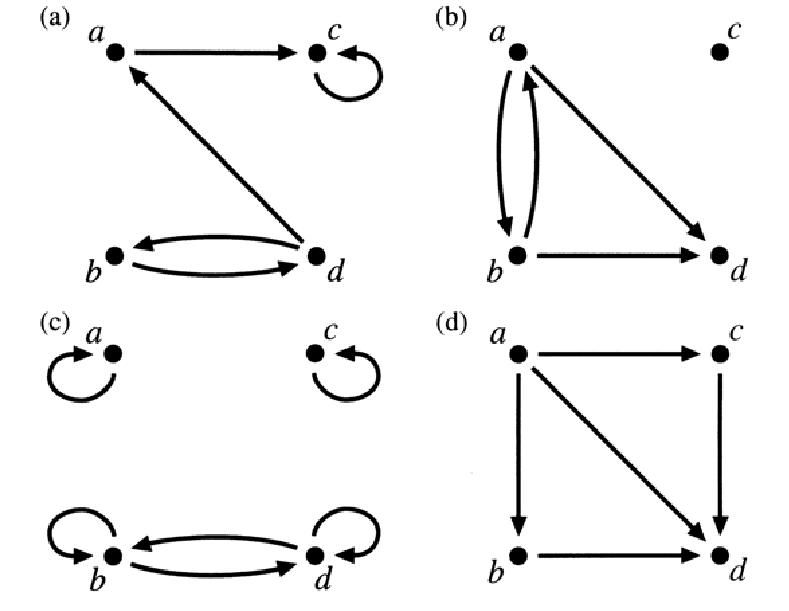
\includegraphics[width=0.5\textwidth]{images/4.3_4.png} 
\end{figure}

\textbf{Solution (a):}

\[R = \{(a, c), (d, a), (d, b), (b, d)\}\]
Reflexive: NO, Symmetric: NO, Transitive: NO

\textbf{Solution (b):}

\[R = \{(a, d), (b, d), (b, a), (a, b)\}\]
Reflexive: NO, Symmetric: NO, Transitive: NO

\textbf{Solution (c):}

\[R = \{(a, a), (b, b), (c, c), (d, d), (b, d), (d, b)\}\]
Reflexive: YES, Symmetric: YES, Transitive: YES

\textbf{Solution (d):}

\[R = \{(a, c), (a, b), (a, d), (b, d), (c, d)\}\]
Reflexive: NO, Symmetric: NO, Transitive: YES

\begin{tcolorbox}[title=Problem 5, breakable]
    Figure $4.5$ shows two relations $R$ and $S$. Find $S \circ R$.
\end{tcolorbox}

\begin{figure}[h] 
\centering
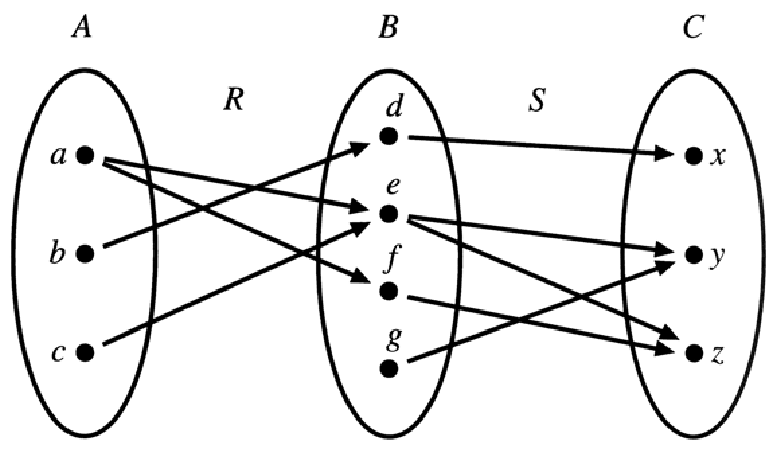
\includegraphics[width=0.5\textwidth]{images/4.3_5.png} 
\end{figure}

\textbf{Solution:}

$S \circ R = \{(a, y), (a, z), (a, z), (b, x), (c, y), (c, z)\}$

\begin{tcolorbox}[title=Problem 7, breakable]
    Prove $R$ is reflexive iff $i_A \subseteq R$,
    where $i_A$ is the identity relation of $A$.
\end{tcolorbox}

\begin{proof}
    ($\rightarrow$) Suppose $R$ is reflexive.
    It follows that for all $x \in A$, $(x, x) \in R$.
    So we can select two arbitrary elements $x, y \in A$
        and if $x = y$ then $(x, y) = (x, x) \in R$.
    Therefore $i_A \subseteq R$.

    ($\leftarrow$) Suppose $i_A \subseteq R$.
    For all $x, y \in A$ where $x = y$, $(x, y) \in R$.
    So we can select two arbitrary elements $x, x \in A$
        and since $x = x$, $(x, x) \in R$.
    Therefore, $R$ is reflexive.
\end{proof}

\begin{tcolorbox}[title=Problem 8, breakable]
    Prove $R$ is transitive iff $R \circ R \subset R$.
\end{tcolorbox}

\begin{proof}
    ($\rightarrow$) Suppose $R$ is transitive.
    So for all $x, y, z \in A$, if $(x, y) \in R$ 
        and $(y, z) \in R$ then $(x, z) \in R$.
    Let $(x, y)$ be an arbitrary pair of elements in $R \circ R$.
    There exists an element $c$ such that $(x, c) \in R$ and $(c, y) \in R$.
    Since $(x, c) \in R$ and $(c, y) \in R$ it follows that $(x, y) \in R$.

    ($\leftarrow$) Suppose $R \circ R \subseteq R$.
    Let $(x, y)$ be an arbitrary pair of elements in $R \circ R$.
    There exists an element $c$ such that $(x, c) \in R$ and $(c, y) \in R$.
    It follows since $R \circ R \subseteq R$ that $(x, y) \in R$.
    Since $(x, y)$ was arbitrary in $R \circ R$, this holds 
        for all $x, y, z \in A$. 
    So if $(x, z) \in R$ and $(z, y) \in R$, then $(x, y) \in R$.
    Therefore, $R$ is transitive.
\end{proof}

\begin{tcolorbox}[title=Problem 9, breakable]
    Suppose $A$ and $B$ are sets.

    (a) Show that for every relation $R$ from $A$ to $B$. $R \circ i_A = R$.

    (b) Show that for every relation $R$ from $A$ to $B$. $i_B \circ R = R$.
\end{tcolorbox}

\begin{proof}
    We first show $R \circ i_A \subseteq R$.
    Let $(x, y)$ be an arbitrary pair of elements in $R \circ i_A$.
    There exists an element $c$ such that $(x, c) \in i_A$ and $(c, y) \in R$.
    But $(x, c) \in i_A$ so $c = x$.
    Therefore $(x, y) \in R$.

    We now show $R \subseteq R \circ i_A$.
    Let $(x, y)$ be an arbitrary pair of elements in $R$.
    We know $(x, x) \in i_A$. 
    Since $(x, x) \in i_A$ and $(x, y) \in R$, $(x, y) \in R \circ i_A$.

    Since $R \circ i_A \subseteq R$ and $R \subseteq R \circ i_A$
        $R \circ i_A = R$.
\end{proof}

\begin{proof}
    We first show $i_B \circ R \subseteq R$.
    Let $(x, y)$ be an arbitrary pair of elements in $i_B \circ R$.
    There exists an element $c$ such that $(x, c) \in R$ and $(c, y) \in i_B$.
    Since $(c, y) \in i_B$, $y = c$.
    Therefore $(x, y) \in R$.

    We now show $R \subseteq i_B \circ R$.
    Let $(x, y)$ be an arbitrary pair of elements in $R$.
    We know $(y, y) \in i_B$.
    Since $(x, y) \in R$ and $(y, y) \in i_B$, $(x, y) \in i_B \circ R$.

    Since $i_B \circ R \subseteq R$ and $R \subseteq i_B \circ R$,
        $i_B \circ R = R$.
\end{proof}

\begin{tcolorbox}[title=Problem 10, breakable]
    Suppose $S$ is a relation on $A$.
    Let $D = Dom(S)$ and $R = Ran(S)$.

    Prove that $i_D \subseteq S^{-1} \circ S$
        and $i_R \subseteq S \circ S^{-1}$.

    Prove that $i_R \subseteq S \circ S^{-1}$.
\end{tcolorbox}

\begin{proof}
    Let $(x, x)$ be an arbitrary pair in $i_D$.
    There exists $y$ such that $(x, y) \in S$.
    Clearly $(y, x) \in S^{-1}$.
    Since $(x, y) \in S$ and $(y, x) \in S^{-1}$ 
        then $(x, x) \in S \circ S^{-1}$.
\end{proof}

\begin{proof}
    Let $(y, y)$ be an arbitrary pair in $i_R$.
    There exists $x$ such that $(x, y) \in S$.
    Clearly $(y, x) \in S^{-1}$.
    Since $(x, y) \in S$ and $(y, x) \in S^{-1}$ 
        then $(y, y) \in S \circ S^{-1}$.
\end{proof}

\begin{tcolorbox}[title=Problem 11, breakable]
    Suppose $R$ is a relation on $A$.
    Prove that if $R$ is reflexive then $R \subseteq R \circ R$.
\end{tcolorbox}

\begin{proof}
    Suppose $R$ is reflexive.
    Let $(x, y)$ be an arbitrary pair in $R$.
    Since $R$ is reflexive $(y, y) \in R$.
    Let $z = y$, then $(x, z) \in R$ and $(z, y) \in R$.
    Therefore $(x, y) \in R \circ R$.
\end{proof}

\begin{tcolorbox}[title=Problem 12, breakable]
    Suppose $R$ is a relation on $A$.

    (a) Prove that if $R$ is reflexive, then so is $R^{-1}$

    (b) Prove that if $R$ is symmetric, then so is $R^{-1}$.

    (c) Prove that if $R$ is transitive, then so is $R^{-1}$.
\end{tcolorbox}

\begin{proof}
    Suppose $R$ is reflexive.
    Let $x$ be an arbitrary element in $A$.
    Since $R$ is reflexive $(x, x) \in R$.
    Since $(x, x) \in R$, $(x, x) \in R^{-1}$.
    Since for all $x \in A$, $(x, x) \in R^{-1}$ it follows that $R^{-1}$ is reflexive.
\end{proof}

\begin{proof}
    Suppose $R$ is symmetric.
    Let $x, y$ be elements in $A$ such that $(x, y) \in R$.
    Since $R$ is symmetric $(y, x) \in R$.
    Since $(x, y) \in R$ then $(y, x) \in R^{-1}$.
    Since $(y, x) \in R$ then $(x, y) \in R^{-1}$.
    Since $(y, x) \in R^{-1}$ and $(x, y) \in R^{-1}$ it follows that
        $R^{-1}$ is symmetric.
\end{proof}

\begin{proof}
    Suppose $R$ is transitive.
    Let $x, y, z$ be arbitrary elements in A such that $(x, y) \in R$
    and $(y, z) \in R$. Since $R$ is transitive $(x, z) \in R$.
    Clearly, $(y, x) \in R^{-1}$, $(z, y) \in R^{-1}$, and $(z, x) \in R^{-1}$.
    Since $(z, x), (z, y), (y, x)\in R^{-1}$ it follows that
        $R^{-1}$ is transitive.
\end{proof}

\begin{tcolorbox}[title=Problem 12, breakable]
    Suppose $R$ is a relation on $A$.

    (a) Prove that if $R$ is reflexive, then so is $R^{-1}$.

    (b) Prove that if $R$ is symmetric, then so is $R^{-1}$.

    (c) Prove that if $R$ is transitive, then so is $R^{-1}$.
\end{tcolorbox}

\begin{proof}    
    Suppose $R$ is reflexive.
    Let $x$ be an arbitrary element in $A$.
    Since $R$ is reflexive $(x, x) \in R$.
    It then follows trivially that $(x, x) \in R^{-1}$.
    Therefore $R^{-1}$ is reflexive.
\end{proof}

\begin{proof}
    Suppose $R$ is symmetric.
    Let $(y, x)$ be an arbitrary element in $R^{-1}$.
    It follows that $(x, y) \in R$.
    Since $R$ is symmetric $(y, x) \in R$.
    It follows that $(x, y) \in R^{-1}$.
    Therefore $R^{-1}$ is symmetric.
\end{proof}

\begin{proof}
    Suppose $R$ is transitive.
    Let $(x, y)$ and $(y, z)$ be arbitrary elements in $R^{-1}$.
    It follows that $(y, x) \in R$ and $(z, y) \in R$.
    Since $R$ is transitive $(z, x) \in R$.
    It follows that $(x, z) \in R^{-1}$.
    Therefore $R^{-1}$ is transitive. 
\end{proof}

\begin{tcolorbox}[title=Problem 13, breakable]
    Suppose $R_1$ and $R_2$ are relations on $A$.
    For each part give either a proof or a counterexample to justify your answer.

    (a) If $R_1$ and $R_2$ are reflexive, must $R_1 \cup R_2$ be reflexive?

    (b) If $R_1$ and $R_2$ are symmetric, must $R_1 \cup R_2$ be symmetric?

    (c) If $R_1$ and $R_2$ are transitive, must $R_1 \cup R_2$ be transitive?
\end{tcolorbox}

\begin{proof}
    Suppose $R_1$ and $R_2$ are reflexive.
    Let $x$ be an arbitrary element in $A$.
    Since $R_1$ and $R_2$ are reflexive it follows that $(x, x) \in R_1$ and $(x, x) \in R_2$.
    It follows that $(x, x) \in R_1 \cup R_2$.
    Therefore $R_1 \cup R_2$ is reflexive.
\end{proof}

\begin{proof}
    Suppose $R_1$ and $R_2$ are symmetric.
    Let $(x, y)$ be an arbitrary element in $R_1 \cup R_2$.
    It follows that $(x, y) \in R_1$ or $(x, y) \in R_2$.
    Suppose $(x, y) \in R_1$.
    Since $R_1$ is symmetric $(y, x) \in R_1$ and therefore $(y, x) \in R_1 \cup R_2$.
    Suppose $(x, y) \in R_2$.
    Since $R_2$ is symmetric $(y, x) \in R_2$ and therefore $(y, x) \in R_1 \cup R_2$.
    Therefore $R_1 \cup R_2$ is symmetric.
\end{proof}

\textbf{Solution:}
\[A = \{1, 2, 3\} \quad R_1 = \{(1, 2)\} \quad R_2 = \{(2, 3)\}\]
\[R_1 \cup R_2 = \{(1, 2), (2, 3)\}\]
Now clearly $R_1$ and $R_2$ are transitive. However, $R_1 \cup R_2$ is not transitive because 
    $(1, 2) \in R_1 \cup R_2$ and $(2, 3) \in R_1 \cup R_2$
    but $(1, 3) \not \in R_1 \cup R_2$

\begin{tcolorbox}[title=Problem 22, breakable]
    Consider the following putative theorem:
    \begin{theorem}
        Suppose $R$ is a relation on $A$. If $R$ is symmetric and 
        transitive, then $R$ is reflexive.
    \end{theorem}
    Is the following proof correct? If so, what proof strategies does it use?
    If not, can it be fixed? Is the theorem correct?
    \begin{proof}
        Let $x$ be an arbitrary element of $A$. Let $y$ be any element of $A$
        such that $xRy$. Since $R$ is symmetric, it follows that $yRx$.
        But then by transitivity, since $xRy$ and $yRx$ we can conclude 
        that $xRx$. Since $x$ was arbitrary, we have shown that $\forall{x} \in A (xRx)$,
        so $R$ is reflexive.
    \end{proof}
\end{tcolorbox}

\textbf{Solution:}

The proof is invalid since it assumes properties about $y \in A$ namely that $x, y \in R$.
The theorem is incorrect so it cannot be fixed.

\begin{tcolorbox}[title=Problem 24, breakable]
    Let $R = \{(m, n) \in \mathbb{N} \times \mathbb{N} \mid |m - n| \le 1\}$,
    which is a relation on $\mathbb{Z}$. This exersize will illustrate
    why, in part $1$ of Definition $4.3.2$, we define the phrase ``$R$ is 
    reflexive on $A$'', rather than simply ``$R$ is reflexive''.
    
    (a) Is $R$ reflexive on $\mathbb{N}$?

    (b) Is $R$ reflexive on $\mathbb{Z}$?
\end{tcolorbox}

\textbf{Solution (a):}

Yes $R$ is reflexive on $\mathbb{N}$. Let $x$ be an arbitrary element in $\mathbb{N}$.
    It follows that $|x - x| = 0 \le 1$ and therefore $(x, x) \in R$.
    
\textbf{Solution (b):} 

Yes $R$ is reflexive on $\mathbb{Z}$. Let $x$ be an arbitrary element in $\mathbb{Z}$.
    It follows that $|x - x| = 0 \le 1$ and therefore $(x, x) \in R$.

\subsection{Ordering Relations}

\begin{tcolorbox}[title=Problem 1, breakable]
    In each case, say whether or not $R$ is a partial order on $A$.
    If so, is it a total order? 

    (a) $A = \{a, b, c\}, R = \{(a, a), (b, a), (b, b), (b, c), (c, c)\}$ 

    (b) $A = \mathbb{R}, R = \{(x, y) \in \mathbb{R} \times \mathbb{R} \mid |x| \le |y|\}$ 

    (c) $A = \mathbb{R}, R = \{(x, y) \in \mathbb{R} \times \mathbb{R} \mid |x| < |y| \text{ or } x = y\}$
\end{tcolorbox}

\textbf{Solution (a):}

$R$ is a partial order on $A$.
$R$ is not a total order on $A$ because $aRc$ and $cRa$ are false.

\textbf{Solution (b):}

$R$ is not a partial order.
Consider $(3, -3)$ so clearly $3R(-3)$ and $(-3)R3$ but $3 \not= -3$.

\textbf{Solution (c):}

$R$ is a partial order on $A$.
$R$ is not a total order because $5R(-5)$ and $(-5)R5$ are false.

\begin{tcolorbox}[title=Problem 2, breakable]
    In each case, say whether or not $R$ is a partial order on $A$. 
    If so, is it a total order? 

    (a) $A =$ the set of all English words.  
    $R = \{(x, y) \in A \times A \mid$  
    where the word $y$ occurs at least as late in alphabetical order as the word $x$$\}$.

    (b) $A =$ the set of all English words.  
    $R = \{(x, y) \in A \times A \mid$  
    where the first letter of the word $y$ occurs at least as late in the alphabet as the first letter of the word $x$$\}$.

    (c) $A =$ the set of all countries in the world.  
    $R = \{(x, y) \in A \times A \mid$  
    where the population of country $y$ is at least as large as the population of country $x$$\}$.
\end{tcolorbox}

\textbf{Solution (a):}

$R$ is a partial order on $A$ and a total order on $A$.

\textbf{Solution (b):}

$R$ is not a partial order on $A$.
Consider ``the'' and ``tip''.
Now ``the''$R$``tip'' and ``tip''$R$``the'' but ``tip''$\not= $``the''.
So $R$ is not antisymmetric.

\textbf{Solution (c)}

$R$ is not a partial order on $A$.
Consider $a =$ America population $100$ and $m =$  Mexico population $100$.
Then $aRm$ and $mRa$ but $a \not= m$ so $R$ is not antisymmetric.

\begin{tcolorbox}[title=Problem 3, breakable]
    In each case find all minimal and maximal elements of $B$.
    Also find, if they exist, the largest and smallest elements of $B$,
    and the least upper bound and greatest lower bound of $B$.

    (a) $R =$ the relation shown in the directed graph in Figure $4.6$,
        $B = \{2, 3, 4\}$.

    (b) $R = \{(x, y \in \mathbb{\mathbb{R}} \times \mathbb{\mathbb{R}} \mid x \le y)\}$,
        $B = \{(x \in \mathbb{R} \mid 1 \le x < 2)\}$.

    (c) $R = \{(x, y) \in \mathcal{P}(\mathbb{N}) \times \mathcal{P}(\mathbb{N}) \mid x \subseteq y\}$,
        $B = \{(x \in \mathcal{P}(\mathbb{N})) \mid \text{$x$ has at most $5$ elements.}\}$
\end{tcolorbox}

\begin{figure}[h] 
\centering
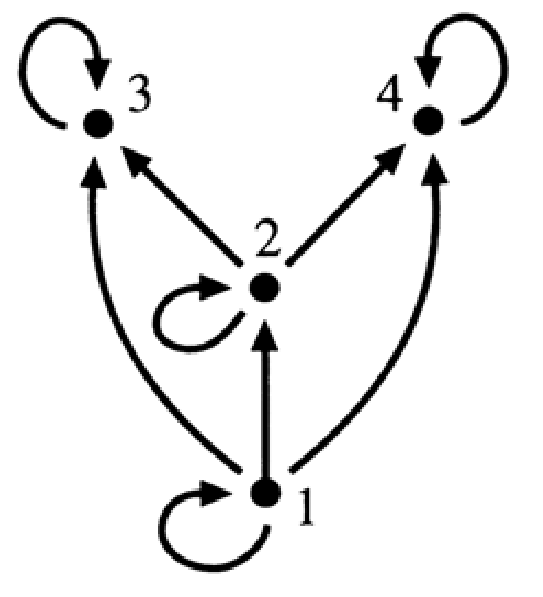
\includegraphics[width=0.3\textwidth]{images/4.4_2.png} 
\end{figure}

\textbf{Solution (a):}

Minimal elements: $\{2\}$, Maximal elements: $\{3, 4\}$

Smallest element: $2$, Largest element: none

Greatest lower bound: $2$, Least upper bound: none

\textbf{Solution (b):}

Minimal elements: $\{1\}$, Maximal elements: none

Smallest element: $1$, Largest element: none

Greatest lower bound: $1$, Least upper bound: $2$

\textbf{Solution (c):}

Minimal elements: $\{\emptyset\}$, Maximal elements: Any $5$ element subset of $\mathbb{N}$

Smallest element: $\emptyset$, Largest element: none

Greatest lower bound: $\emptyset$, Least upper bound: none

\begin{tcolorbox}[title=Problem 4, breakable]
    Suppose $R$ is a relation on $A$. You might think $R$ could not be both 
    antisymmetric and symmetric, but this isn't true. Prove that $R$ is both 
    antisymmetric and symmetric iff $R \subseteq i_A$.
\end{tcolorbox}

\begin{proof}
    ($\rightarrow$) Suppose $R$ is both antisymmetric and symmetric.
    Let $x$, $y$ be arbitrary elements in $A$ such that $xRy$.
    Since $R$ is symmetric and $xRy$ it follows that $yRx$.
    Then, since $R$ is antisymmetric and $xRy$ and $yRx$, it follows that $x = y$.
    Therefore $(x, y) = (x, x) \in i_A$.

    ($\leftarrow$) Suppose $R \subseteq i_A$.
    Let $x$, $y$ be arbitrary elements in $A$ such that $xRy$.
    Since $R \subseteq i_A$ it follows that $(x, y) \in i_A$ and therefore $x = y$.
    So $xRy$ and $yRx$ implies $x = y$ so $R$ is antisymmetric.
    Also, $xRy$ implies $yRx$ so $R$ is symmetric.

    Thus $R$ is both antisymmetric and symmetric iff $R \subseteq i_A$.
\end{proof}

\begin{tcolorbox}[title=Problem 6, breakable]
    Suppose $R_1$ and $R_2$ are partial orders on $A$.
    For each part, give either a proof or a counterexample to justify your answer.

    (a) Must $R_1 \cap R_2$ be a partial order on $A$?

    (b) Must $R_1 \cup R_2$ be a partial order on $A$?
\end{tcolorbox}

\begin{proof}
    To prove that $R_1 \cap R_2$ is a partial order on $A$,
        we must show it is reflexive, antisymmetric, and transitive on $A$.
    First note that $R_1$, $R_2$ being partial orders on $A$ implies that 
        they are reflexive, antisymmetric, and transitive on $A$.

    We first show $R_1 \cap R_2$ is reflexive.
    Let $x$ be an arbitrary element in $A$.
    Since $R_1$, $R_2$ are reflexive on $A$ it follows that $xR_1x$ and $xR_2x$.
    It then follows that $x(R_1 \cap R_2)x$.
    Therefore $R_1 \cap R_2$ is reflexive.

    We now show $R_1 \cap R_2$ is antisymmetric.
    Let $x$, $y$ be arbitrary elements in $A$ such that $x(R_1 \cap R_2)y$
        and $y(R_1 \cap R_2)x$.
    This implies $xR_1y$ and $yR_1x$.
    Since $R_1$ is antisymmetric it follows that $y = x$.
    A similar argument shows $y = x$ on $R_2$.
    Therefore $R_1 \cap R_2$ is antisymmetric.

    Finally, we show $R_1 \cap R_2$ is transitive.
    Suppose $x$, $y$, $z$ are arbitrary elements in $A$ such that $x(R_1 \cap R_2)y$
        and $y(R_1 \cap R_2)z$.
    It follows that $xR_1y$ and $yR_1z$.
    Since $R_1$ is transitive it follows that $xR_1z$.
    A similar argument shows $xR_2z$.
    Therefore $R_1 \cap R_2$ is transitive.

    Since $R_1 \cap R_2$ is reflexive, antisymmetric, and transitive,
         it is a partial order on $A$.
\end{proof}

\textbf{Solution (b):}

\[A = \{1, 2, 3\} \quad R_1 = \{(1, 1), (2, 2), (3, 3), (1, 2)\} \quad R_2 = \{(1, 1), (2, 2), (3, 3) (2, 3)\}\]
\[R_1 \cup R_2 = \{(1, 1), (2, 2), (3, 3), (1, 2), (2, 3)\}\]

Notice $1(R_1 \cup R_2)2$ and $2(R_1 \cup R_2)3$ but not $1(R_1 \cup R_2)3$
    therefore $R_1 \cup R_2$ is not transitive and not a partial order.

\begin{tcolorbox}[title=Problem 13, breakable]
    Suppose $R$ is a partial order on $A$. Prove that $R^{-1}$
    is also a partial order on $A$. If $R$ is a total order,
    will $R^{-1}$ also be a total order?
\end{tcolorbox}

\begin{proof}
    Suppose $R$ is a partial order on $A$.

    Let $x$ be an arbitrary element in $A$.
    Since $R$ is a partial order it is reflexive therefore $xRx$.
    But $xRx$ implies $xR^{-1}x$ so $R^{-1}$ is reflexive.

    Let $x$, $y$ be arbitrary elements in $A$ such that $xR^{-1}y$ and $yR^{-1}x$.
    Since $xR^{-1}y$, $yR^{-1}x$ it follows that $yRx$, $xRy$.
    Since $R$ is a partial order it is antisymmetric therefore since $yRx$, $xRy$
        it follows that $x = y$.
    Thus $xR^{-1}y$ and $yR^{-1}x$ implies $x = y$ so $R^{-1}$ is antisymmetric.

    Let $x$, $y$, $z$ be arbitrary elements in $A$ such that $xR^{-1}y$ and $yR^{-1}z$.
    Since $xR^{-1}y$, $yR^{-1}z$ it follows that $yRx$, $zRy$.
    Since $R$ is a partial order it is transitive therefore since $zRy$, $yRx$
        it follows that $zRx$ and therefore $xR^{-1}z$.
    Thus $xR^{-1}y$ and $yR^{-1}z$ implies $xR^{-1}z$ so $R^{-1}$ is transitive.

    Since $R^{-1}$ was reflexive, antisymmetric, and transitive it is a partial order.
\end{proof}

\textbf{Solution (b):}

By the previous proof if $R$ is a total order than $R^{-1}$ is at least a partial order.
Now, $R$ being a total order implies for all $x$, $y$ either $xRy$ or $yRx$.
Clearly either $yR^{-1}x$ or $xR^{-1}y$ is true in that case therefore $R^{-1}$ is 
also a total order.

\begin{tcolorbox}[title=Problem 14, breakable]
    Suppose $R$ is a partial order on $A$, $B \subseteq A$, and $b \in B$.
    Exersize $13$ shows that $R^{-1}$ is also a partial order on $A$.

    (a) Prove that $b$ is the $R$-largest element of $B$ iff it is the $R^{-1}$-smallest
        element of $B$.

    (b) Prove that $b$ is an $R$-maximal element of $B$ iff it is an $R^{-1}$-minimal 
        element of $B$.
\end{tcolorbox}

\begin{proof}
    ($\rightarrow$) Suppose that $b$ is an $R$-largest element of $B$.
    So for all $a \in B$, $aRb$. 
    It then follows that $bR^{-1}a$.
    Since $a$ was arbitrary, for all $a \in B$, $bR^{-1}a$. 
    So $b$ is the $R^{-1}$-smallest element of $B$.

    ($\leftarrow$) The argument is symmetrical.

    Therefore $b$ is the $R$-largest element of $B$ iff it is the $R^{-1}$-smallest
        element of $B$.
\end{proof}

\begin{proof}
    ($\rightarrow$) Suppose that $b$ is an $R$-maximal element of $B$.
    There does not exist $a \in B$ such that $bRa$ and $b \not= a$.
    So there does not exist $a \in B$ such that $aR^{-1}b$ and $a \not= b$.
    Therefore $b$ is the $R^{-1}$-minimal element of $B$.

    ($\leftarrow$) The argument is symmetrical.

    Therefore $b$ is an $R$-maximal element of $B$ iff it is an $R^{-1}$-minimal 
        element of $B$.
\end{proof}

\begin{tcolorbox}[title=Problem 19, breakable]
    Consider the following putative theorem. \\

    \textbf{Theorem} Suppose $R$ is a total order on $A$ and $B \subset A$.
    Then every element of $B$ is either the smallest element of $B$
    or the largest element of $B$. \\

    (a) What's wrong with the following proof of the theorem? \\
    \begin{proof}
        Suppose $b \in B$. Let $x$ be an arbitrary element of $B$.
        Since $R$ is a total order, either $bRx$ or $xRb$.

        Case $1$. $bRx$. Since $x$ was arbitrary, we can conclude that 
        $\forall{x} \in B(bRx)$, so $b$ is the smallest element of $R$.

        Case $2$. $xRb$. Since $x$ was arbitrary, we can conclude that 
        $\forall{x} \in B(xRb)$, so $b$ is the largest element of $R$.

        Thus, $b$ is either the smallest element of $B$ or the largest element 
        of $B$. Since $b$ was arbitrary, every element of $B$ is either its 
        smallest element or its largest element.
    \end{proof}

    (b) Is the theorem correct? Justify your answer with either a proof 
        or a counterexample.
\end{tcolorbox}

\textbf{Solution (a):}

Within each case $x$ is not an arbitrary element of $B$.
The issue is $x$ has an additional property that $bRx$ in case $1$
and $xRb$ in case $2$.

\textbf{Solution (b):}

The theorem is incorrect. Consider the following counterexample:
\[A = \mathbb{N}, B = \{1, 2, 3\}, R = \{(x, y) \in A \times A \mid x \le y\}\]
Clearly $2$ is not the R-largest element since $(2, 3) \in R$ and $2 \not= 3$.
But $2$ is also not the R-smallest element since $(1, 2) \in R$ and $1 \not= 2$.

\begin{tcolorbox}[title=Problem 23, breakable]
    Prove Theorem $4.4.11$.

    \textbf{Theorem $4.4.11$} Suppose $A$ is a set $\mathcal{F} \subseteq \mathcal{P}(A)$,
    and $\mathcal{F} \not= \emptyset$. Then the least upper 
    bound of $\mathcal{F}$ (in the subset partial order) is $\bigcup\mathcal{F}$
    and the greatest lower bound of $\mathcal{F}$ is $\bigcap\mathcal{F}$.
\end{tcolorbox}

\begin{proof}
    Suppose $A$ is a set $\mathcal{F}\subseteq\mathcal{P}(A)$, and $\mathcal{F} \not= \emptyset$.
    Clearly $\bigcup\mathcal{F}$ is an upper bound 
        since for all $A \in \mathcal{F}$ if $x \in A$ then  $x \in \bigcup \mathcal{F}$.
    It follows that $A \subseteq \bigcup \mathcal{F}$ showing that $\bigcup \mathcal{F}$ is an upper bound.
    For contradiction, suppose $B \in \mathcal{F}$ and 
        $B \not= \bigcup \mathcal{F}$ and $B$ is the \emph{l.u.b}.
    Either $B \not \subseteq \bigcup \mathcal{F}$ of $\bigcup \mathcal{F} \not \subseteq b$.

    Suppose $B \not \subseteq \bigcup \mathcal{F}$. This would imply $B$ is not an upper 
    bound which is a contradiction.

    Suppose $\bigcup \mathcal{F} \not \subseteq B$. But for all 
        for all $A \in \mathcal{F}$ if $x \in A$ then  $x \in \bigcup \mathcal{F}$.
    Contradicting that $B \in \mathcal{F}$.

    Therefore $\bigcup \mathcal{F}$ is the \emph{l.u.b}.
\end{proof}

\begin{tcolorbox}[title=Problem 24, breakable]
    Suppose $R$ is a relation on $A$. Let $S = R \cup R^{-1}$.

    (a) Show that $S$ is a symmetric relation on $A$ and $R \subseteq S$.

    (b) Show that if $T$ is symmetric relation on $A$ and $R \subseteq T$
        then $S \subseteq T$.

    Note that this exersize shows that $S$ is the smallest element of the set 
    $\mathcal{F} = \{T \subseteq A \times A \mid R \subseteq T \text{ and } T \textbf{ is symmetric}\}$;
    in other words, it is the smallest symmetric relation on $A$ that contains $R$ as a subset. This 
    relation $S$ is called the symmetric closure of $R$.
\end{tcolorbox}

\begin{tcolorbox}[title=Problem 25, breakable]
    Suppose that $R$ is a relation on $A$. Let $\mathcal{F} = \{T \subseteq A \times A \mid R \subseteq T
    \text{ and } T \text{ is transitive}\}$.

    (a) Show that $\mathcal{F} = \emptyset$.

    (b) Show that $\bigcap \mathcal{F}$ is a transitive relation on $A$ and $R \subseteq \bigcap \mathcal{F}$.
    
    (c) Show that $\bigcap \mathcal{F}$ is the smallest transitive relation on $A$ that contains $R$ 
        as a subset. The relation $\bigcap \mathcal{F}$ is called the transitive closure of $R$.
\end{tcolorbox}

\begin{tcolorbox}[title=Problem 26, breakable]
    Suppose $R_1$ and $R_2$ are relations on $A$, and let $R_1 \subseteq R_2$.

    (a) Let $S_1$ and $S_2$ be the symmetric closures of $R_1$ and $R_2$,
        respectively. Prove that $S_1 \subseteq S_2$. (See exersize $24$ for the 
        definition of symmetric closure.)

    (b) Let $T_1$ and $T_2$ be the transitive closures of $R_1$ and $R_2$, respectively.
        Prove that $T_1 \subseteq T_2$. (See exersize $25$ for the definition of transitive
        closure.)
\end{tcolorbox}

\begin{tcolorbox}[title=Problem 27, breakable]
    Suppose $R_1$ and $R_2$ are relations on $A$, and let $R = R_1 \cup R_2$.

    (a) Let $S_1$, $S_2$, and $S$ be symmetric closures of $R_1$, $R_2$, and $R$,
        respectively. Prove that $S_1 \cup S_2 = S$. (See exersize $24$ for the definition
        of symmetric closure.)

    (b) Let $T_1$, $T_2$, and $T$ be the transitive closures of $R_1$, $R_2$, and $R$,
        respectively. Prove that $T_1 \cup T_2 \subseteq T$, and give an example to 
        show that it may happen that $T_1 \cup T_2 \not= T$. (See exersize $25$ for 
        the definition of transitive closure.)
\end{tcolorbox}

\begin{tcolorbox}[title=Problem 28, breakable]
    Suppose $A$ is a set.

    (a) Prove that if $A$ has at least two elements then there is no largest antisymmetric
        relation on $A$. In other words, there is no relation $R$ on $A$ such that 
        $R$ is antisymmetric, and for every antisymmetric relation $S$ on $A$, $S \subseteq R$.

    (b) Suppose $R$ is a total order on $A$. Prove that $R$ is a maximal antisymmetric relation 
        on $A$. In other words, there is no antisymmetric relation $S$ on $A$ such that $R \subseteq S$
        and $R \not= S$.
\end{tcolorbox}

\begin{tcolorbox}[title=Problem 30, breakable]
    Suppose $R$ is a relation on $A$, and let $T$ be the transitive closure of $R$.
    Prove that if $R$ is symmetric, then so is $T$. (Hint: Assume that $R$ is symmetric.
    Prove that $R \subseteq T^{-1}$ and $T^{-1}$ is transitive. What can you conclude 
    about $T$ and $T^{-1}$? See exersize $25$ for the definition of transitive closure.)
\end{tcolorbox}
